\chapter{Aufgabe D1}
Im Folgenden wird die Tabelle der 3-Punkt-Abschätzung dargestellt. Die Aufgabe D2 \glqq Analyse der einzelnen Signale"' beanspruchte mehr Zeit als geplant. Die Aufgaben mit ASCET konnten häufig nur in der \glqq pessimistisch"' geschätzen Zeit durchgeführt werden. Hier wurde häufig zu wenig Zeit eingeplant, um Probleme mit dem Programm ASCET zu lösen. Die Zusatzaufgabe D13* liegt weit unter der geschätzten Zeit, da hier nur ein Ansatz ausgearbeitet aber nicht umgesetzt wurde.\\

\begin{figure}[h!]
	\centering
	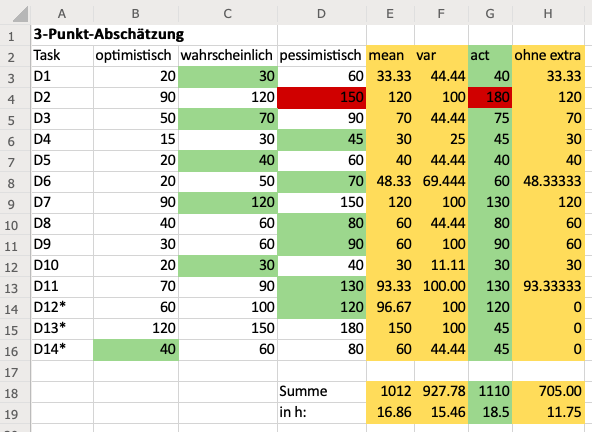
\includegraphics[width=1\linewidth]{../Graphiken/Schaetzung.png}
	\caption{3-Punkt-Abschätzung}
	\label{fig:schaetzung}
\end{figure}